\documentclass[11pt]{article}
\usepackage[english]{babel}

\usepackage{caption}
\usepackage{helvet}


\usepackage{amsmath}
\usepackage{color}
\usepackage{amssymb}

\usepackage{graphicx}
\usepackage{soul}
\usepackage{cite}
\usepackage{fancyhdr}
\usepackage{wrapfig}
%%%%My Packages%%%%
\usepackage{subcaption}
\usepackage{textcomp}
\usepackage{comment}


\newcommand{\ga}{\alpha}
\newcommand{\gb}{\beta}
\newcommand{\gam}{\gamma}
\newcommand{\gd}{\delta}
\newcommand{\eps}{\epsilon}
\newcommand{\veps}{\varepsilon}
\newcommand{\gz}{\zeta}

\newcommand{\gt}{\theta}
\newcommand{\gi}{\iota}
\newcommand{\gk}{\kappa}
\newcommand{\gl}{\lambda}
\newcommand{\gs}{\sigma}
\newcommand{\go}{\omega}
\newcommand{\Gam}{\Gamma}
\newcommand{\gD}{\Delta}
\newcommand{\gT}{\Theta}
\newcommand{\gL}{\Lambda}
\newcommand{\gS}{\Sigma}
\newcommand{\gO}{\Omega}

 
%%%%%%%%%

\newcommand{\pt}[1]{\left( #1\right)}
\newcommand{\pq}[1]{\left[ #1 \right]}
\newcommand{\pg}[1]{\left\{ #1\right\}}
\newcommand{\figref}[1]{\figurename~\ref{#1}}
\newcommand{\red}[1]{\textcolor{red}{#1}}
\newcommand{\blue}[1]{\textcolor{blue}{#1}}

\usepackage{changepage}
\changepage{5.8cm}{6cm}{0cm}{-3.0cm}{0cm}{-2.9cm}{0cm}{-0.5cm}{-0.5cm}
%{length of the text}{width of the text}{even side margin}{odd side margin}
%{column sep}{topmargin}{headhight}{headsep}{from text to pagenumber}
\pagestyle{fancy}
\lfoot{\footnotesize  2Pmod2}
%\chead{\bf Origins of life}
\rhead{\footnotesize \today}
\lhead{\footnotesize Eliza Guseva}
\chead{Two Polymer Model}
\rfoot[]{\thepage}
\renewcommand{\footrulewidth}{0.4pt}
% Remove brackets from numbering in List of References
\makeatletter
%\renewcommand{\@biblabel}[1]{\quad#1.}
\makeatother
\renewcommand{\indexname}{Notations}
\renewcommand{\familydefault}{\sfdefault}

\begin{document}
 \begin{center}
  {\Large \textbf{Ken's view on life's origin}}
 \end{center}
\paragraph{Disclaimer.} Ken didn't see this graphics yes. So this is more like my view on Ken's views.
\begin{itemize}
 \item Legend to Petri Nets diagrams, which I'm using here
\begin{figure}[h!]
 \centering
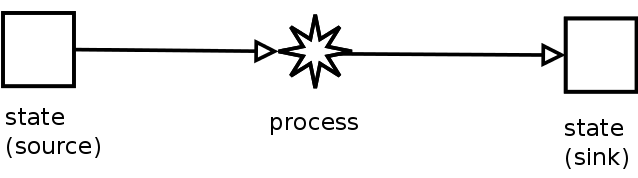
\includegraphics[width=0.35\textwidth]{legend.png}
\end{figure}
\item Good. (Machines get destroyed faster than Blueprints)
\begin{figure}[h!]
 \centering
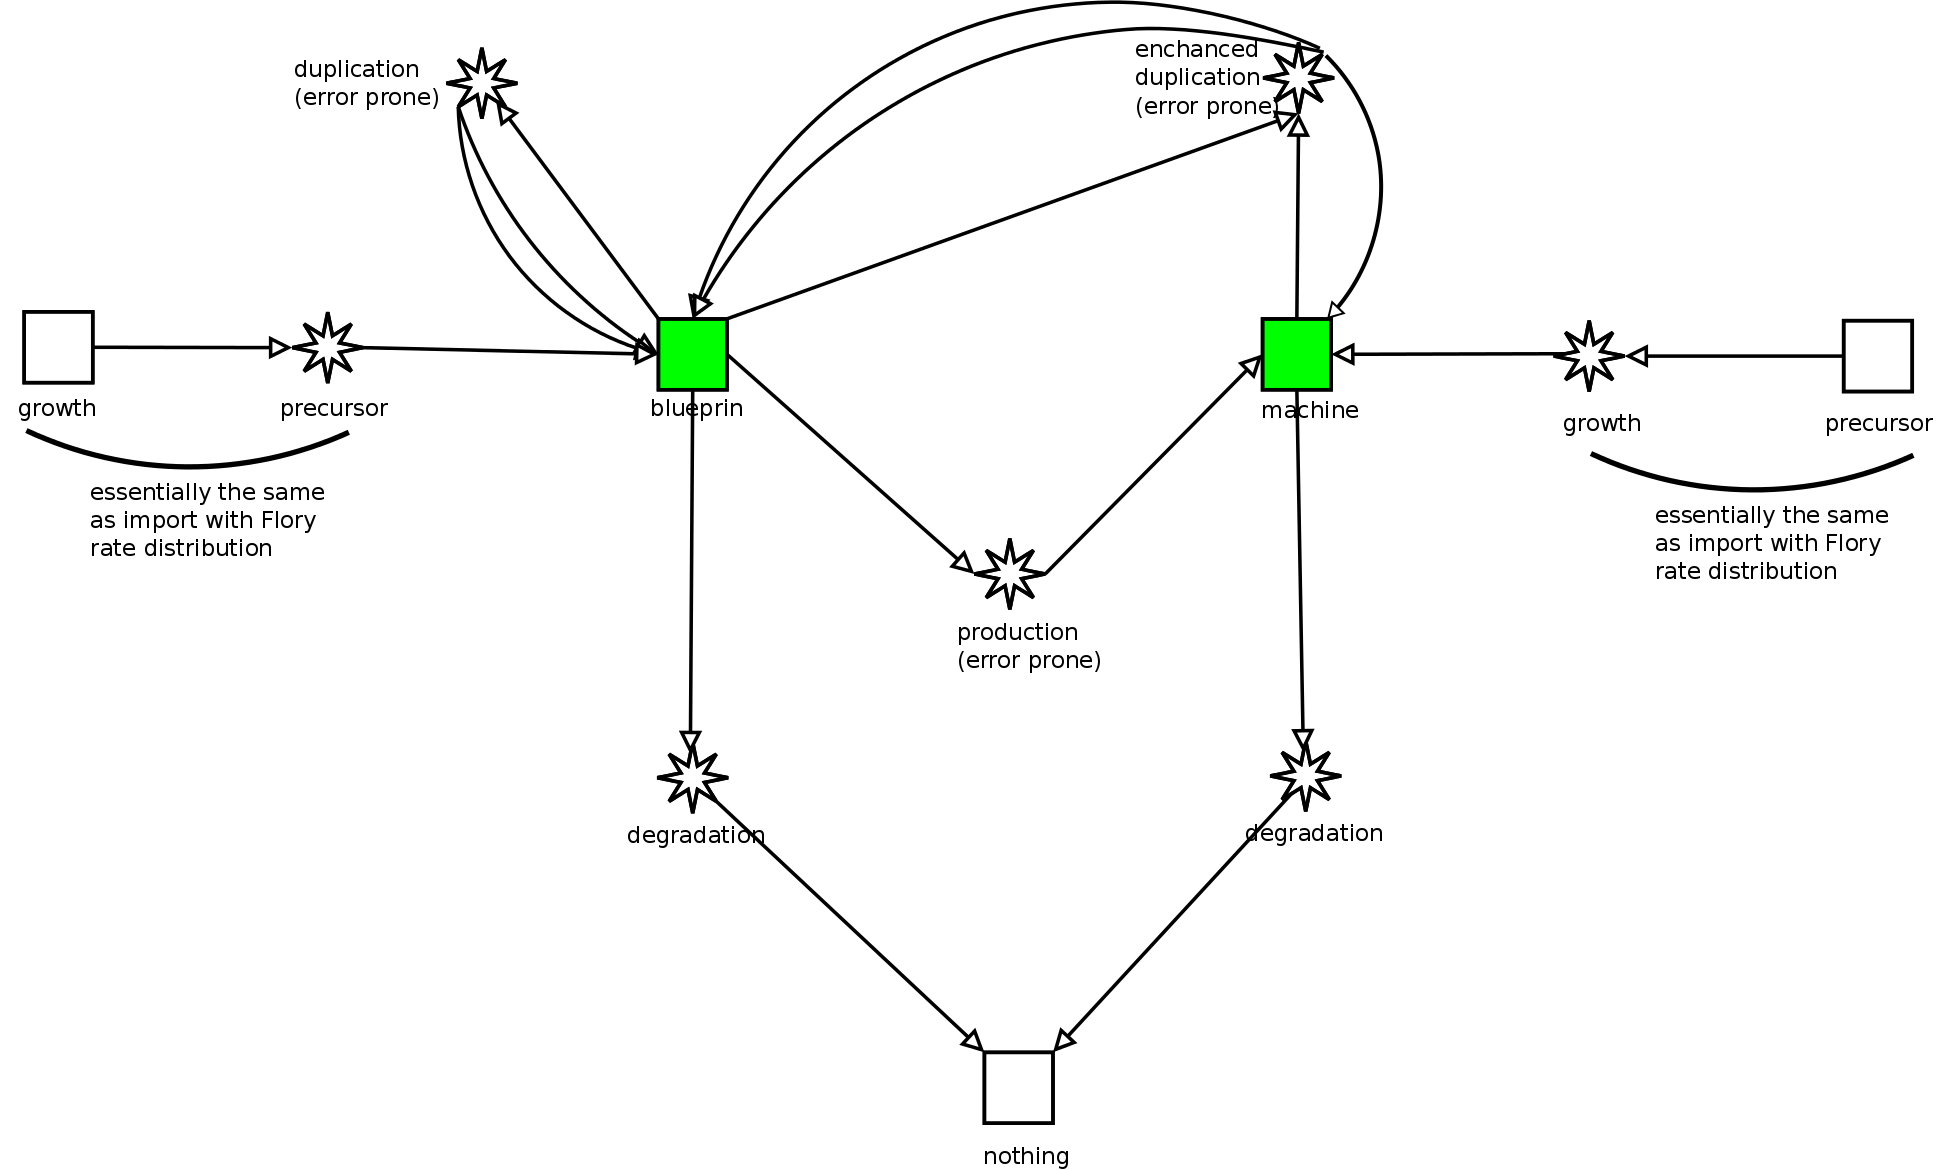
\includegraphics[width=0.99\textwidth]{blueprint-machine.png}
\end{figure}

\item Bad. 
\begin{figure}[h!]
 \centering
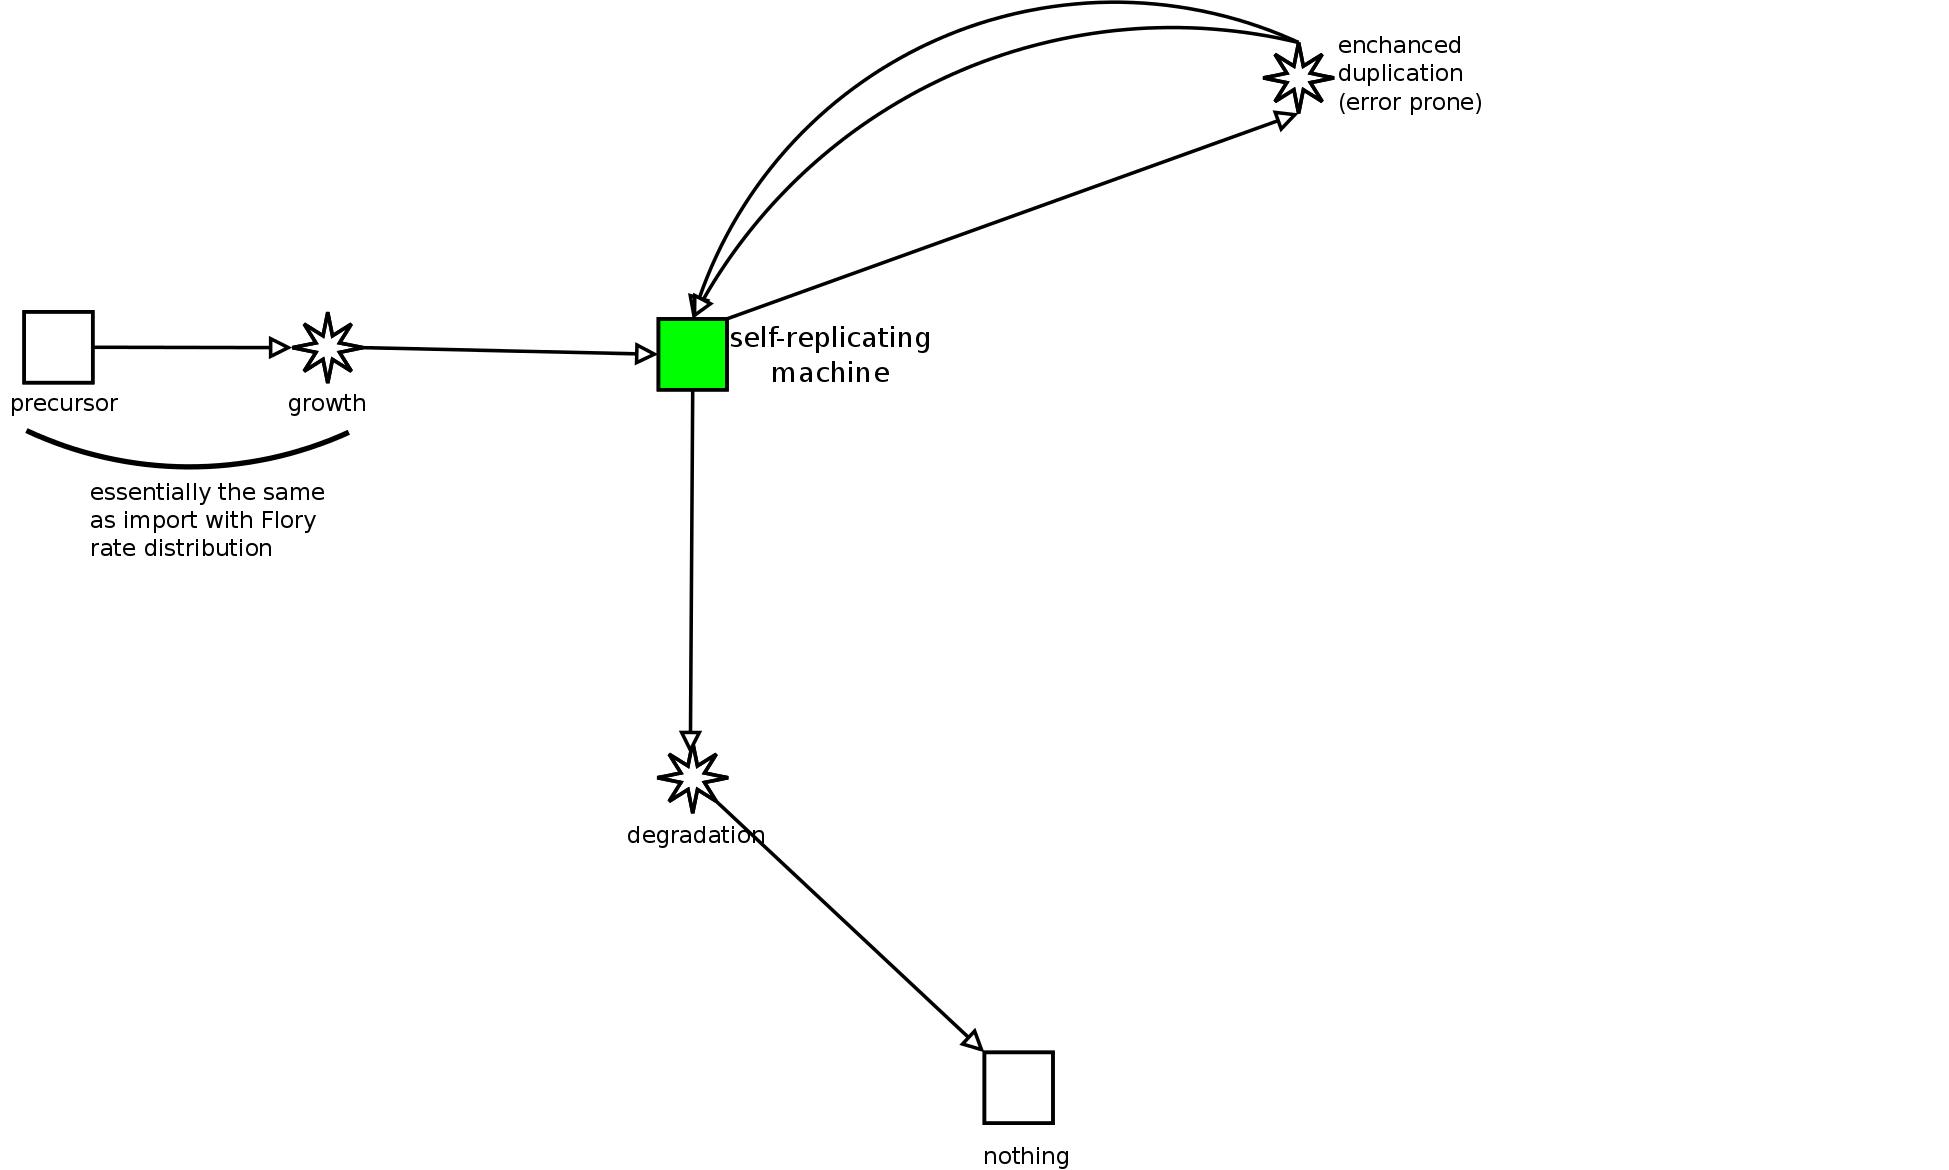
\includegraphics[width=0.99\textwidth]{selfreplicating-machine.png}
\end{figure}
\end{itemize}




\end{document}
